\chapter{Design and Implementation}\label{C:workdone}

\section{Overview}

The goal of the project as mentioned in Section \ref{C:intro} is to create a tool to allow developers to identify redundant test cases. The tool is split into several different sections and the chapter will discuss each. The first objective of the tool was to trace the test data. We explore two different frameworks and compare the usability of each. After the tool was able to trace the data, we determine what spectra we are interested in. These are then discussed. The next section then discusses using edit distance metrics to compare test case trace information. Throughout the testing of the tool, one of the main impediments was the time taken to analyse the large amount of data. We examine how breaking the analysis into a series of pipeline stages decreases the time taken.

\section{Tracing}
\label{S:trace}
A fundamental requirement for this project was to trace the methods executed by a test. David Pearce's language Whiley is written in Java, therefore it was decided to use Java frameworks to trace the tests. There were two tracing framework's considered. The first framework considered was AspectJ. The technique that AspectJ uses is Aspect Oriented Programming (AOP). AOP can be used to add code to an existing program without modifying the source code. To distinguish what code to weave, and where in the existing code to weave it, AspectJ uses a \textit{pointcut} \cite{aspectj}. An \textit{aspect} contains multiple point cuts. Weaving the aspect can be achieved through the following methods:

\begin{itemize}
\item \textbf{Compile time} --
The classes are compiled with the aspect woven into them. When the program is executed, the methods have the code from the aspect woven into them already. This requires the source to be compiled with AspectJ's compiler.
\item \textbf{Load time} --
The weaving process is deferred until the point at which a class loader attempts to load in a class file. Load time modification is achieved by using a command line argument notifying Java to use the AspectJ class loader.
\end{itemize}

The other framework we considered was the Java Debugging Interface (JDI). JDI is similar to using an observer pattern. It selects a list of classes to observe and when a method within a selected class is called, the listener class is notified. This class is then passed the information about the method call. 

AspectJ provided several advantages over JDI. The ability to choose which methods to record was easier to define and it returns the actual object when retrieving the parameters of the method call. This detail becomes important when we explore tracing parameter values in Section \ref{parameterTrace}. In comparison, JDI was faster to execute, however there was a limited amount of documentation available and the parameters returned were not the actual objects. The decision to use AspectJ was based off this trade off between information and performance. Decoupling the data gathering and data analysis within the tool removed the emphasis on retrieval performance. This meant that the tracing performance was less of an issue.

Our pointcuts record every method execution. Figure \ref{fig:aspectused} shows a simplified version. There are two pointcuts within the aspect. The first pointcut gets called for every method call which has a JUnit \@Test annotation attached to it. This will then call a static service passing it the method information of the new test. The second pointcut traces everything apart from the methods with a JUnit \@Test annotation attached. It then passes the information to the static service. The next stage was to weave the aspect into a benchmark. Using compile time weaving would have meant that every benchmark had to be recompiled using the aspect compiler. In contrast, load time only requires the AspectJ class loader to be passed through a command line argument. Load time was chosen as it was easy to use when working with external benchmarks.

\begin{figure}[h]
\begin{center}
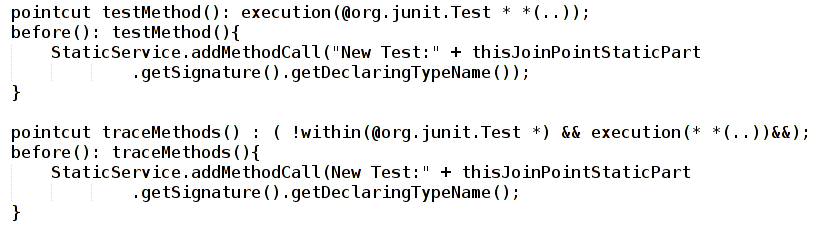
\includegraphics[width = \textwidth]{aspect.png}
\end{center}
\caption{A simplified pointcut within AspectJ. The first pointcut is for when a new test is executed and the second when a new method is executed.}
\label{fig:aspectused}
\end{figure}

\subsection{Saving to the Network}
To execute the analysis on a grid computing system, the test data had to be accessible on the School of Engineering's local network. To achieve this, the trace data was saved to the local network. Not only did it allow for the analysis to be executed on the grid system, it also it allowed for the data to be reanalysed without having to re trace the test suite. 

\section{Filtering By Spectra }
\label{S:spectra}
The idea of a spectrum was previously identified in Chapter \ref{C:intro}. Reexamining the idea, a spectrum is some abstraction of the method information. There are three different types of spectrum. These are \textit{unique method calls}, \textit{all method calls} and \textit{call tree}, each with its own characteristic. It is important to understand how we use a spectra. When the tool is tracing the tests, it traces the amount of information needed based on a settings file. A spectra can then be applied to this trace information to filter out data to match the spectra's characteristic. The tool ensures that the traced information is able to be filtered by the spectrum. 

We will examine the spectra characteristics in relation to the example shown in Figure \ref{fig:callingexample}. The different spectra take up different levels of resources, these are are: time taken and memory. 


\begin{figure}[h]
\begin{center}
\includegraphics[height = 6cm]{callingexample.png}
\end{center}
\caption{A simple representation of a call tree of three that is traced from a test. Each letter represents a method call and the bold letter is the active method in each line of the call tree.}
\label{fig:callingexample}
\end{figure}

\subsection{Unique Method Calls}
The ``unique method call" spectrum filters out the repetition of methods. The data after applying the filter only has each method represented a single time. The motivation of this spectrum is to substantially reduce the time taken and memory used. Consequently, decreasing the amount of data leads to a decrease in the confidence that the tests identified are truly redundant. 

Examining Figure \ref{fig:callingexample}, on the left hand side are the method calls where each line represents one call. The active method is in bold and the parent methods are before it. On the right hand side is the call tree. With no filtering applied the method calls are ``A,B,C,D,C,B,D". When we apply a ``unique method calls" spectrum filter, the data will become ``A,B,C,D". This shows that we are filtering out a large portion of data while retaining an adequate representation of the original trace information. We can explore how this affects the Whiley Compiler benchmark. There are 494 unique methods called for a particular test and 80,000 method executions. Utilising the unique method call spectrum, the tool will only use 494 method executions when comparing the test with another, rather than the 80,000. This is $\rfrac{6}{1000}$ of the original amount. 

\subsection{All Method Calls}
The ``all method calls" spectrum filters out information regarding the call tree. The motivation behind this approach is to analyse a larger subset of trace data than the ``unique method calls" spectrum. Comparing the two, ``all method calls" increases our confidence in the results however, this increases the time taken and memory used to analyse the information.

Examining Figure \ref{fig:callingexample}, the output of filtering the method calls with this spectrum would be ``A,B,C,D,C,B,D". This shows a loss of the context data. We can explore how this effects the Whiley Compiler benchmark. When using an ``all method calls" spectrum, the tool will use all 80,000 method executions when comparing the test with another.

\subsection{Call Tree}
A ``call tree" may filter out some of the parent methods. The number of calls retained is referred to as the K depth \cite{Zhuang06accurate}. The motivation behind the approach is to increase our confidence in the results by taking into account the \textit{context} of a call. The consequence of increasing the amount of data is a further increase in the time taken and memory used to analyse the trace data in comparison to the other two spectra.

We can filter the Figure \ref{fig:callingexample} using a K depth of two. This would lead to the filtered data returning 'A, A $\rightarrow$ B', 'B $\rightarrow$ C', 'A $\rightarrow$ D', 'D $\rightarrow$ C', 'A $\rightarrow$ B' and 'B $\rightarrow$ D'. We can see that by using a K depth of two, we lose some of the information from the trace data. To stop this loss of data, we could extend the depth to three. Using the Whiley Compiler benchmark as an example, a call tree filter would examine all 80,000 method executions. The difference with the "all method calls" filter is that each execution contains a total of three calls.

To retrieve the calling context in Java, the current stack trace of a method call is examined. It is then parsed to retrieve the relevant information. This parsing involves removing the method calls that are used to retrieve the stack trace and any memory location details. 

\section{Analysis Metrics}
\label{S:metrics}
Having traced the information and being able to filter out specific data. This filtered data needs to be then compared with another test cases data to produce a redundant level between them. Edit distance metrics were choosen to perform this comparison. They were discussed in Section \ref{editdistbg}, with two different edit distance metrics considered. They were: Monge \& Elkan \cite{monge1997efficient} which splits the strings into sections and compares the sections and Levenshtein \cite{levenshtein1966binary} which compares tokens that are generally single characters. 

For both of the algorithms, there were publicly available frameworks that implemented them. Both implementations allowed for a call tree to be represented by a token. The trace information of the test cases were represented by a list of tokens. The issue with Monge \& Elkan was it attempted to find the best match with no regard to the ordering. Attempting to find the best match would increase the time taken, perform unnecessary computation for our requirements and increase the false positive rate. The trace information in Figure \ref{fig:mongevleven} can be used to show the difference between the metrics. The implementation of Monge \& Elkan would match 'Method Call' in test case 1 to the 'Method Call' in test case 2, even though they were called at different times. Levenshtein did not search for a match, rather the metric only looked at the opposing method call. This direct matching was preferred as we were interested in the order of the method calls as well as what methods were called.

\begin{figure}[h]
\begin{center}
\includegraphics[width = \textwidth]{MongeVLeven.png}
\end{center}
\caption{Trace information used to show the difference between Monge \& Elkan and Levenshtein metric implementations. The Monge \& Elkan metric will disregard ordering and measure these test cases as being the same. The Levenshtein metric examines one to one and will measure the test cases as having no similarities.}
\label{fig:mongevleven}
\end{figure}

\section{Pipeline }
\label{pipelinesection}
For the tool to help developers reduce the number of redundant tests, it has to analyse the information within an acceptable time frame. Comparing every test with every other while using all the available information (e.g. call tree) in some cases resulted in the analysis taking several days to complete. This is not considered an acceptable time frame. This issue arises when each of the spectrum of the test cases contain tens of thousands of method calls. A pipeline approach was implemented to get around this issue of lengthy analysis. Figure \ref{fig:pipeline} visualises the idea. The figure shows the trace information is input into the start of the pipeline. The purpose of a stage is to determine the redundancy of test pairs. If a pair is more redundant than amount specified, it will be stored and analysed during the next stage. The goal is that each subsequent stage should soundly eliminate pairs from consideration that the next stage would have removed. Heuristics can help achieve this goal. A heuristic would examine a subset of data while still eliminating test pairs that would have been removed in the subsequent stages. 

\begin{figure}[h]
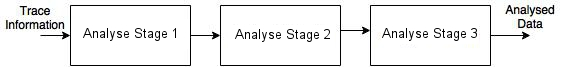
\includegraphics[width=\textwidth]{Pipeline.jpg}
\caption{Trace information goes in at the start of the pipeline. After each stage there should be a reduction of comparisons that the next stage has to complete. The last stage should be the most computationally heavy.}
\label{fig:pipeline}
\end{figure}

To further expand on the heuristic idea, the tool can use the spectra filters to examine the trace information in different perspectives. The particular filter of interest is the ``unique method calls" spectrum. Inspecting a subset of the trace data increased the speed of the comparison but as a consequence, it decreased the confidence of the output being truly redundant. We can increase the confidence by then analysing the output test pairs with a ``context tree" filter. An important part to emphasize is that no information is lost when information is filtered, rather some of it is ignored for that pipeline stage only. We see a pipeline set up in Figure \ref{fig:pipelineExample}. The first stage uses a ``unique method calls" spectrum and pipelines the output into a ``call tree" of depth thee. The three test cases at the top are the trace information input into the pipeline. The remainder of this section explores this example. 

\paragraph{Pipeline Stage 1}
The tool first filters the trace information with a ``unique method call" spectrum (Single method A and Z ignored). The three test cases are filtered into:

\begin{enumerate}
\item ``B,C,D" 
\item ``E,H,J,M,Q"
\item ``B,C,D"
\end{enumerate}

Calculating the Levenshtein distance between each, it would show that test cases 1 and 3 are similar but test case 2 has no similarities to either. The test cases that are passed onto the next pipeline stage are test cases 1 and 3.

\paragraph{Pipeline Stage 2}

The information used in this stage is shown at the top of the figure. The only test cases compared are test cases 1 and 3. Looking at the test cases, when filtered with a call tree of depth three there are no similarities between the two method calls. This is because that highest level calls are different between them. Hence the output of the pipeline as a whole is that there are no redundant test cases in the trace information.

\begin{figure}[h]
\includegraphics[width=\textwidth]{callingexampleExtra.png}
\caption{A two stage pipeline that analyses the trace information shown. The first stage uses a ``unique method calls" filter with a 98\% similarity and the second stage filters with a call tree of K Depth three with a 98\% similarity. After analysing the data, no test cases are returned as being redundant.}
\label{fig:pipelineExample}
\end{figure}

An alternative heuristic to use is the ``all method calls" spectrum. In comparison to the ``unique method calls" filter, the ``all method calls" filter further decreases the amount of comparisons that the final pipeline does. It then leads to an increase in confidence of the results but also, an increase in the time taken and memory consumption. This approach may be used as the last stage in a pipeline of the length two. The other option, would be to have it as the middle stage in a pipeline of length three.

\section{Tracing Parameter Values}
\label{parameterTrace}
The related work in this research area has explored using statement coverage while ignoring the parameter values of each method. It could be argued that due to knowing the statement path, parameters are irrelevant as you know the path the method will take, and parameters do not add any more information. When tracing at the method level rather than at the statement level, parameters become crucial to determine the degree of redundancy between test cases. This is because parameters give insight into the execution paths that will be taken and act as a proxy to the statement information without storing the same amount of the data.

There were two variations of parameters that were considered to trace. Firstly, primitive types only. Primitives only represented a small number of parameters when running pre-experiments on the benchmarks.  The parameters collected had a limited effect on the number of false positives identified and time taken. The second approach was to use reflection. Reflection is the ability to examine and modify objects at run time \cite{oraclereflection}. Since AspectJ gives direct access to the object's within the method parameters, reflection can be used. By using reflection, we retrieve the fields of the object and return them in a string to represent the state of the object. If there are objects within the object, a reference is returned to ensure no cycles occur. This string is then examined to remove any Java reference locations and then stored. The reflection is done through the Apache commons language library. We decided to use reflection as it was more representative of a method call in comparison to primitive types only.

The most common use case of the tool is expected to use parameters. We therefore decided to optimize this through storing the data with them. The optimization involved saving the parameters directly onto the method executions. If parameters were not required, they have to be split off rather than being concatenated on. This leads to an increase in the set up time.

\section{Weighting }
Maurer et al. \cite{koochakzadeh2009test} and Robinson et al. \cite{li2008static} found that test suites often had a set of methods that were in every test case, such as setup and tear down. These common methods could create false positives. To understand why, a redundant test is one where it is nearly or exactly a replication of another test. Since each method call within a spectra has the same weighting, the more setup and teardown calls made means that the exercise stage has decreased weighting overall. We can see an example of this in Figure \ref{fig:weightingdiagram}. The figure shows test cases with different proportions of setup and tear down in relation to the exercise stage. It also shows how the size of the test case may have different proportions. This is when a test suite contains both large and small test cases that use the same setup and teardown methods. The figure shows that this would cause the small test case to have an increased portion of setup and teardown methods.

Two different variations of weighting were considered. The first variation involved giving each method execution a weighting based on its call frequency, the higher the frequency, the lower the weighting. This would cause the more common methods to have less impact on the final result, but not be completely removed. The other variation that was considered, and used, was completely removing the most used method calls for each test case. This involved determining method calls that were called 80\% or more than the most frequent. This approach allowed us to remove only high frequent calls. The method executions to these calls were then removed at the start of the pipeline stage. During initial experiments, the first variation had less impact. The reason was that the frequent method calls were still having a large effect, even with a lower weighting. This meant that each benchmark needed to use different weightings, therefore it was difficult to find a solution that could be applied on every benchmark. This variation was applied on a per test case level and is referred to as weighting technique throughout the remainder of the report.

\begin{figure}[h]
\includegraphics[width= \textwidth, height=6cm]{weightingdiagram.png}
\caption{A diagram showing how the different size of the test case can be affected by setup and teardown methods. The ``Exercise" refers to the core test method calls. The figure shows the case where a test suite contains both large and small test cases that use the same setup and teardown methods. It shows that this would cause the small test case would be made up of a larger portion of setup and tear down in comparison to the large test.}
\label{fig:weightingdiagram}
\end{figure}

\section{Summary}

The tool implemented has a range of abilities to achieve the goal of identifying redundant tests in a test suite. To identify redundant tests, the tool can trace the information of a test suite. The analysis can then be executed on this trace information with some settings selected by the user. The user can determine the pipeline, call tree depth, whether to analyse parameters and whether weighting is applied. The redundant tests are then output for the user to inspect and determine the appropriate action. 